% Metódy inžinierskej práce

\documentclass[10pt,twoside,slovak,a4paper]{article}

\usepackage[slovak]{babel}
%\usepackage[T1]{fontenc}
\usepackage[IL2]{fontenc} % lepšia sadzba písmena Ľ než v T1
\usepackage[utf8]{inputenc}
\usepackage{graphicx}
\usepackage{url} % príkaz \url na formátovanie URL
\usepackage{hyperref} % odkazy v texte budú aktívne (pri niektorých triedach dokumentov spôsobuje posun textu)
\usepackage{pdfpages}

\usepackage{cite}
%\usepackage{times}

\pagestyle{headings}

\title{UML Diagramy\thanks{Semestrálny projekt v predmete Metódy inžinierskej práce, ak. rok 2021/22, vedenie: Ing. Ján Lúčanský}} % meno a priezvisko vyučujúceho na cvičeniach

\author{Kristián Lukacsovics\\[2pt]
    {\small Slovenská technická univerzita v Bratislave}\\
    {\small Fakulta informatiky a informačných technológií}\\
    {\small \texttt{xlukacsovics@stuba.sk}}
    }

\date{\small 07. september 2021} % upravte



\begin{document}

\maketitle

\begin{abstract}
\ldots % ...
\end{abstract}



\section{Úvod}

Motivujte čitateľa a vysvetlite, o čom píšete. Úvod sa väčšinou nedelí na časti.

Uveďte explicitne štruktúru článku. Tu je nejaký príklad.
Základný problém, ktorý bol naznačený v úvode, je podrobnejšie vysvetlený v časti~\ref{nejaka}.
Dôležité súvislosti sú uvedené v častiach~\ref{dolezita} a~\ref{dolezitejsia}.
Záverečné poznámky prináša časť~\ref{zaver}.

\section{Nejaká časť 1} \label{nejaka}
\section{Nejaká časť 2} \label{dolezita}
\section{Nejaká časť 3} \label{dolezitejsia}
\section{Nejaká časť 4} \label{zaver}

% 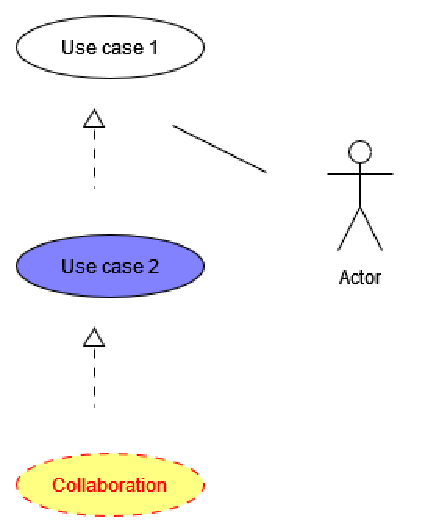
\includegraphics[scale=0.82]{../test_diagram.pdf}
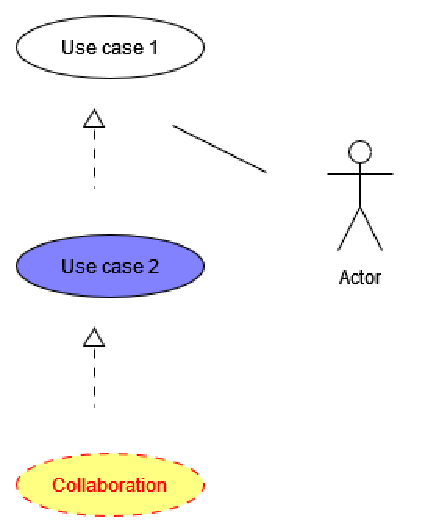
\includepdf[scale=0.2, pages=-]{../test_diagram.pdf} % To include all the pages in the PDF file:

%\acknowledgement{Ak niekomu chcete poďakovať\ldots}


% týmto sa generuje zoznam literatúry z obsahu súboru literature.bib podľa toho, na čo sa v článku odkazujete
\bibliography{literature}
\bibliographystyle{plain} % prípadne alpha, abbrv alebo hociktorý iný
\end{document}
